\documentclass[11pt, a4paper]{article}
\usepackage[utf8]{inputenc}
\usepackage{geometry}
\geometry{margin=1in}
\usepackage{graphicx}
\usepackage{float}
\usepackage{hyperref}
\usepackage{caption}
\usepackage{subcaption}
\usepackage{booktabs}
\usepackage{amsmath}
\usepackage[table]{xcolor}
\definecolor{posgreen}{RGB}{34, 197, 94}
\definecolor{negred}{RGB}{239, 68, 68}

\title{\textbf{The Holy Grail of Finance}\\ \Large Constructing a Robust Fund of Hedge Funds via Uncorrelated Strategies}
\author{Athenee}
\date{\today}

\begin{document}
\maketitle

\section{Introduction: The Core Philosophy}
The ``Holy Grail'' of finance, a concept popularized by Ray Dalio, revolves around a simple yet extraordinarily powerful mathematical truth: combining uncorrelated, positive-returning strategies exponentially improves risk-adjusted returns. In traditional investing, market beta often dictates the majority of portfolio performance. Our approach fundamentally deviates from this by systematically identifying and allocating capital to niche, uncorrelated strategies.

This report outlines the motivation behind our Fund of Hedge Funds (FoF) product. We aim to construct an equal-weighted portfolio of distinct hedge funds. By doing so, we effectively neutralize idiosyncratic and systemic volatility, crushing the portfolio's overall volatility and Maximum Drawdown (MDD) while preserving the underlying aggregate returns. 

The report proceeds as follows: First, we explore the theoretical basis of this phenomenon through Monte Carlo simulations. Second, we empirically validate this using data from the J.P. Morgan Hedge Fund platform. Finally, we discuss our rigorous sourcing and selection methodology for constructing the actual portfolio.

\section{Theoretical Framework: The Power of Diversification}

To illustrate the raw power of diversification, we begin with a theoretical Monte Carlo simulation. Consider a benchmark asset akin to the S\&P 500, possessing a mean annualized return of 10\% and an annualized volatility of 18\%. Over a 10-year horizon, simulated wealth paths reveal a median Maximum Drawdown (MDD) of roughly 30\%, with a 25th percentile MDD of 40\%. 

What if we could find $N$ independent, completely uncorrelated assets with the exact same return (10\%) and volatility (18\%) profile?

By equal-weighting these $N$ assets with monthly rebalancing, the portfolio's expected return remains 10\%, but the volatility scales down proportionally to $1/\sqrt{N}$. With 10 such independent assets, the portfolio volatility shrinks to approximately $5.7\%$.

More impressively, the tail risks are drastically reduced. As shown in Figure \ref{fig:theoretical}, as the number of uncorrelated strategies ($N$) increases, the Maximum Drawdown collapses. For $N=10$, the median MDD on a 10-year horizon drops to around 5\%, representing a 5.5x to 6x reduction compared to a single asset. 

\begin{figure}[H]
    \centering
    \begin{subfigure}[b]{0.45\textwidth}
        \centering
        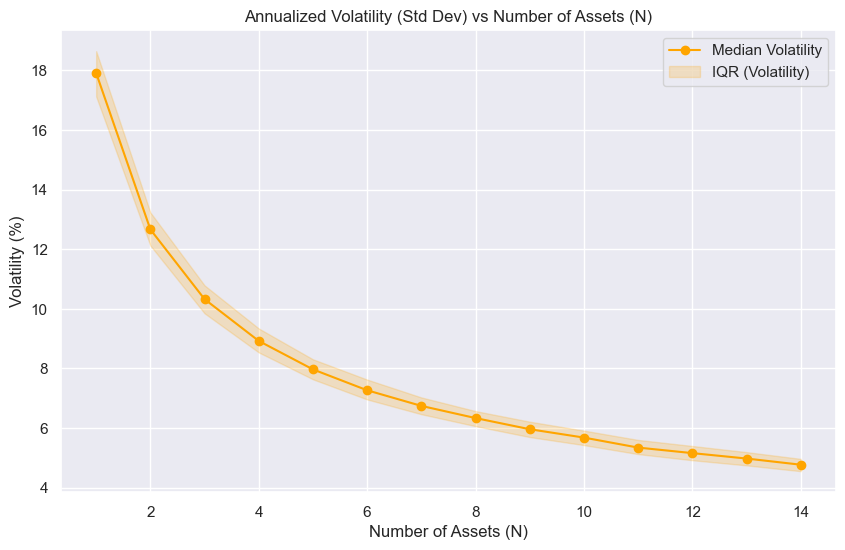
\includegraphics[width=\textwidth]{Theoretical_vol_vs_N.png}
        \caption{Volatility vs. Number of Assets (N)}
    \end{subfigure}
    \hfill
    \begin{subfigure}[b]{0.45\textwidth}
        \centering
        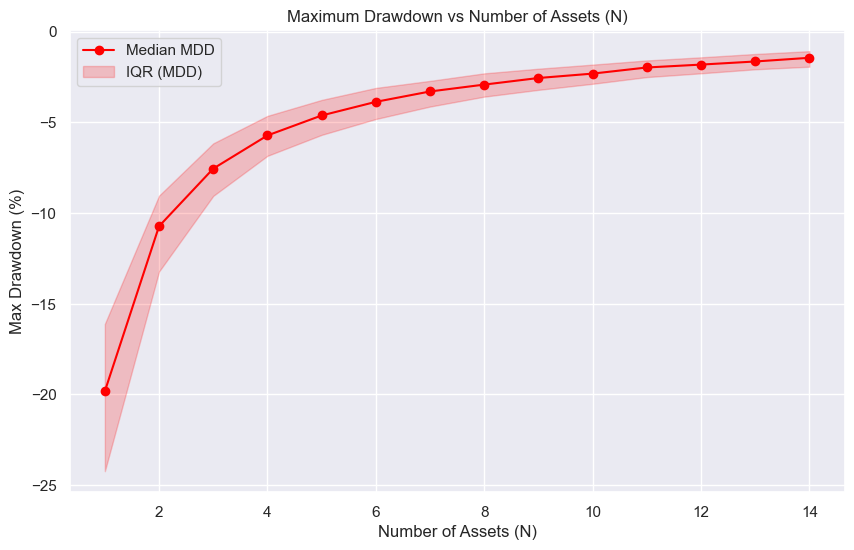
\includegraphics[width=\textwidth]{Theoretical_MDD_vs_N.png}
        \caption{Maximum Drawdown vs. N}
    \end{subfigure}
    \caption{Theoretical Monte Carlo simulations demonstrating the rapid decay of portfolio volatility and Maximum Drawdown as the number of uncorrelated assets ($N$) increases.}
    \label{fig:theoretical}
\end{figure}

This theoretical exercise proves that if one can source truly uncorrelated positive expectancy strategies, the resulting portfolio is structurally superior on a risk-adjusted basis.

\section{Empirical Validation: The J.P. Morgan Universe}

Skeptics often argue that finding truly uncorrelated hedge funds is impossible, and that correlations inevitably spike to 1 during market crises. To address this, we conducted an empirical study on a database of over 800 hedge funds from the J.P. Morgan Cap Intro platform.

We split the data into a training period (2020--2022) and an out-of-sample testing period (2023--2026). During the training period, we selected a subset of top-performing funds based on specific criteria (e.g., top 25\% by Sharpe Ratio), resulting in a pool of eligible funds.

From this pool, we repeatedly sampled $N=10$ funds at random to form equal-weighted portfolios, and then tracked their performance through the out-of-sample period. This Monte Carlo approach allowed us to assess whether ex-ante selection criteria yield genuinely diversified and robust portfolios ex-post.

\begin{figure}[H]
    \centering
    \begin{subfigure}[b]{0.45\textwidth}
        \centering
        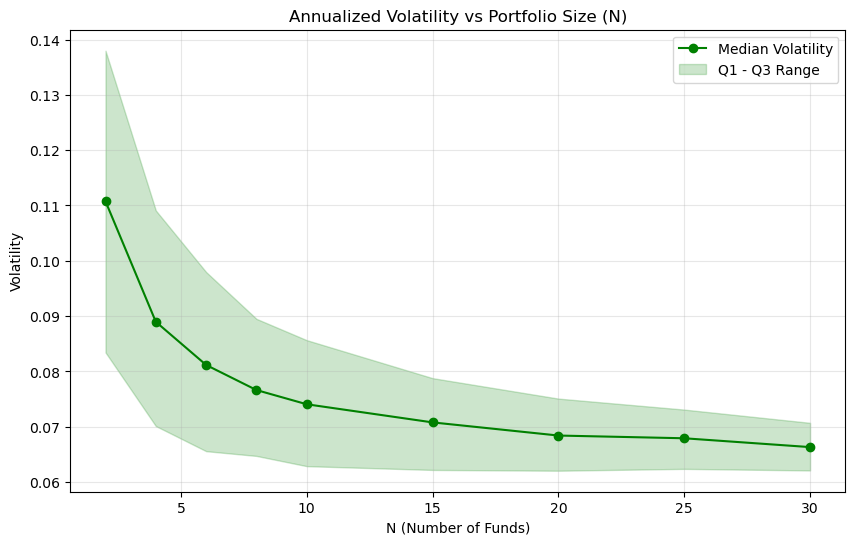
\includegraphics[width=\textwidth]{JPM_vol_stat_N_augmenting.png}
        \caption{Empirical Volatility Reduction}
    \end{subfigure}
    \hfill
    \begin{subfigure}[b]{0.45\textwidth}
        \centering
        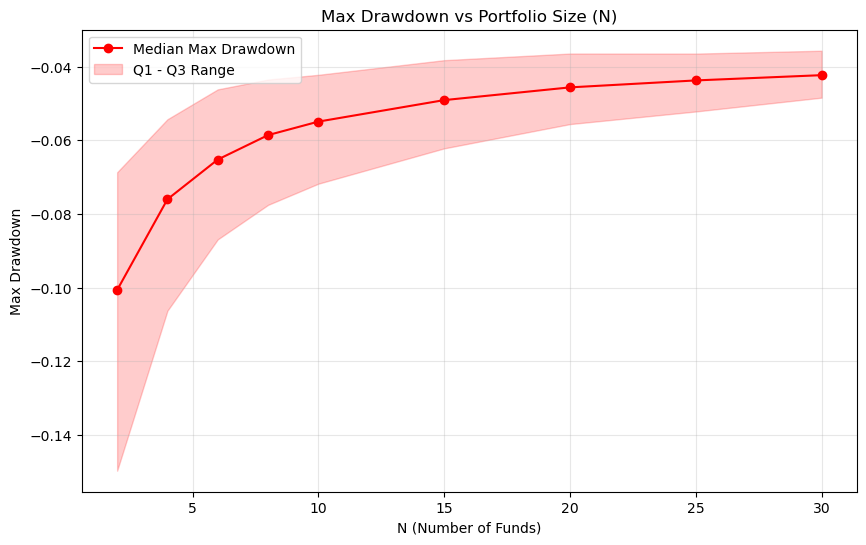
\includegraphics[width=\textwidth]{JPM_MDD_stat_N_augmenting.png}
        \caption{Empirical MDD Reduction}
    \end{subfigure}
    \caption{Empirical statistics for simulated $N$-asset portfolios drawn from top-quartile JPM funds.}
    \label{fig:jpm_stats}
\end{figure}

\begin{figure}[H]
    \centering
    \begin{subfigure}[b]{0.45\textwidth}
        \centering
        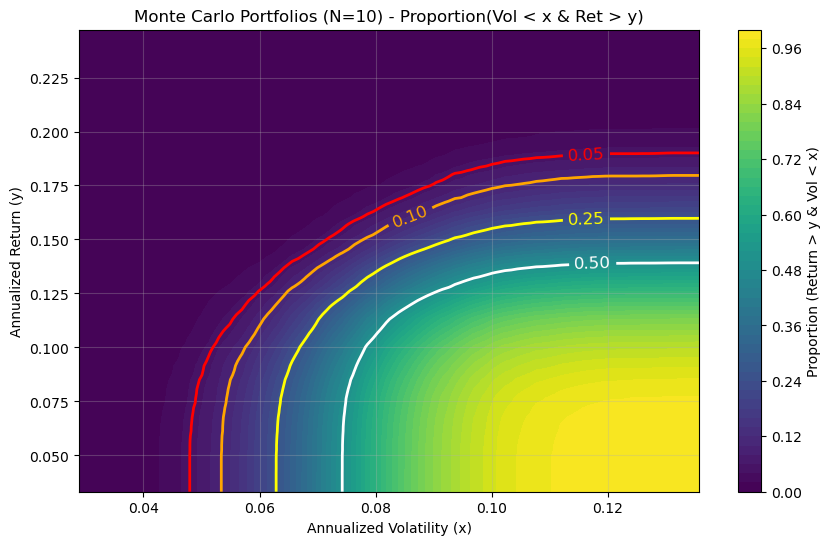
\includegraphics[width=\textwidth]{JPM_vol_ret_surface_N_10.png}
        \caption{Return vs. Volatility Surface}
    \end{subfigure}
    \hfill
    \begin{subfigure}[b]{0.45\textwidth}
        \centering
        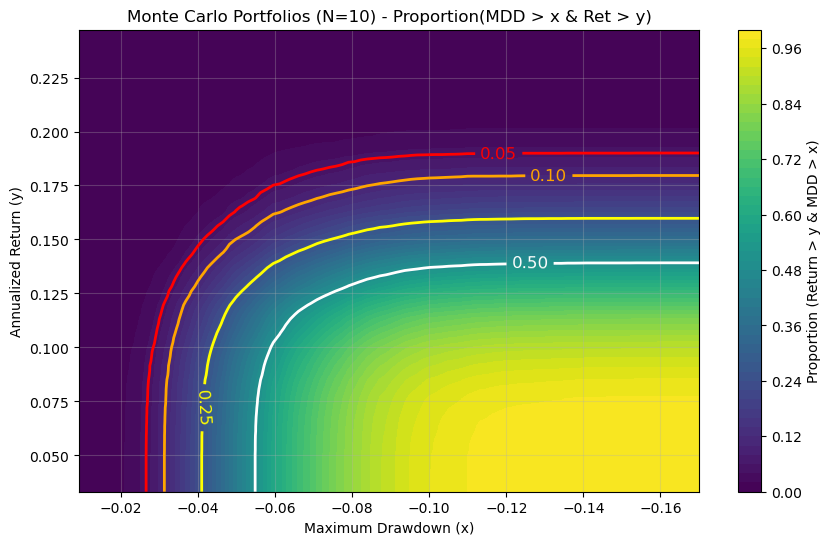
\includegraphics[width=\textwidth]{JPM_MDD_ret_surface_N_10.png}
        \caption{Return vs. MDD Surface}
    \end{subfigure}
    \caption{Probability surfaces of Return vs Volatility and MDD for $N=10$ portfolios.}
    \label{fig:jpm_surfaces}
\end{figure}

The empirical evidence strongly corroborates our theoretical framework. Figures \ref{fig:jpm_stats} and \ref{fig:jpm_surfaces} demonstrate that volatility and MDD are systematically managed downward as $N$ increases. The probability surfaces allow us to quantify the ex-ante risk; for instance, the top 10\% of randomly drawn portfolios exhibit tightly constrained volatility while maintaining impressive returns. Our proprietary selection process is designed to consistently place our FoF within the top decile of these simulated outcomes.

\section{Fund Sourcing and Selection Methodology}

Understanding that diversification is powerful is only the first step; the execution relies entirely on sourcing and selecting the right underlying funds. 

\subsection{Sourcing}
We partner with top-tier Prime Brokerage Capital Introduction teams across major institutions (J.P. Morgan, Société Générale, BNP Paribas, Barclays, Citi, UBS, Goldman Sachs) and specialized third-party marketers. Through over 150 dedicated meetings with Hedge Fund Managers, we have mapped the universe of niche, capacity-constrained strategies.

\subsection{Manager Selection Criteria}
We specifically look for profiles that inherently mitigate systemic risk:
\begin{itemize}
    \item \textbf{Risk Management First:} PMs must have a strict ``Drawdown budget.'' We favor spin-offs from major proprietary trading desks or top-tier pod shops (e.g., Millennium) where brutal risk management (5--7\% drawdown limits) is deeply ingrained.
    \item \textbf{Market Neutrality:} We require purely market-neutral construction. We avoid managers who rely on market timing or directional beta, as this is exceedingly difficult to distinguish from luck.
    \item \textbf{High Turnover \& Niche Markets:} We prefer strategies with high turnover in niche, capacity-constrained markets. High frequency of trades allows us to rapidly determine the statistical significance of a manager's edge.
\end{itemize}

\subsection{Quantitative Filtering}
To ensure true non-correlation, we employ strict quantitative filters:
\begin{itemize}
    \item \textbf{Crisis Alpha:} Performance during the worst decile of S\&P 500 returns must be resilient.
    \item \textbf{Alpha/Beta Profile:} We demand statistically significant Alpha ($t$-statistic $> 2$) and a Beta as close to 0 as possible. Exceptions are occasionally made for slight beta (e.g., 0.2) if the annualized Alpha is exceptionally high ($>20\%$).
    \item \textbf{Low Correlation:} Pairwise correlations to the equity market and to other funds in our portfolio must strictly reside between $-0.2$ and $0.2$.
    \item \textbf{Asymmetric Capture:} We look for inverted upside vs. downside capture ratios (e.g., 0.5 upside vs $-0.5$ downside).
\end{itemize}

\section{Target Portfolio Example: Project Lazarus}

To synthesize the impact of our selection and diversification process, let us project our target portfolio using real, carefully curated funds from the current market environment. The following empirical results dynamically pull from our live ``Project Lazarus'' simulation.

\subsection{Underlying Fund Statistics}

Below are the aggregated statistics of the specific niche hedge funds selected for this portfolio. Each fund has been rigorously vetted for its lack of beta correlation, positive alpha generation, and robust risk management.

\begin{table}[H]
    \centering
    \resizebox{\textwidth}{!}{%
    \begin{tabular}{lrrrrrrrrrrrr}
\toprule
\bfseries Strategy & \bfseries CAGR & \bfseries Std & \bfseries Proxy Sharpe & \bfseries MDD & \bfseries Calmar & \bfseries Pos Months & \bfseries Up Capture & \bfseries Down Capture & \bfseries Alpha (t-stat) & \bfseries Beta & \bfseries Corr SP500 & \bfseries N Months \\
\midrule
Crypto Carry & 18.37\% & 5.43\% & 3.16 & -0.77\% & 23.91 & 92.5\% & 0.43 & -0.41 & 15.81\% (4.79) & 0.06 & 0.15 & 40 \\
Quant FX & 34.62\% & 18.63\% & 1.70 & -26.03\% & 1.33 & 69.6\% & 0.68 & -0.75 & 34.33\% (5.44) & -0.17 & -0.14 & 112 \\
Chinese MN & 20.55\% & 13.63\% & 1.45 & -10.84\% & 1.90 & 65.2\% & 0.39 & -0.60 & 20.53\% (4.86) & -0.06 & -0.06 & 135 \\
Distr Debt & 25.85\% & 11.81\% & 2.02 & -8.74\% & 2.96 & 78.1\% & 0.68 & -0.03 & 20.12\% (4.08) & 0.19 & 0.26 & 73 \\
Quant HFT & 21.33\% & 6.81\% & 2.89 & -1.39\% & 15.35 & 85.7\% & 0.45 & -0.68 & 20.33\% (4.01) & -0.03 & -0.05 & 28 \\
Syst Multi Asset & 47.09\% & 6.60\% & 5.97 & -0.63\% & 74.74 & 97.0\% & 0.79 & -1.06 & 39.92\% (13.68) & -0.03 & -0.08 & 67 \\
Quant Indian & 24.90\% & 7.36\% & 3.09 & -2.20\% & 11.33 & 84.4\% & 0.44 & -0.62 & 24.14\% (7.39) & -0.10 & -0.20 & 64 \\
Biotech & 34.92\% & 15.60\% & 2.02 & -10.63\% & 3.28 & 74.4\% & 0.88 & -0.18 & 26.38\% (4.60) & 0.31 & 0.34 & 86 \\
FX Swap Arbitrage & 29.08\% & 2.06\% & 12.53 & 0.00\% & - & 100.0\% & 0.64 & -0.85 & 26.17\% (17.36) & -0.02 & -0.12 & 27 \\
Quant Global Macro & 46.93\% & 14.41\% & 2.78 & -15.19\% & 3.09 & 86.9\% & 1.15 & -0.58 & 36.08\% (10.14) & 0.28 & 0.28 & 198 \\
\bottomrule
\end{tabular}

    }
    \caption{Performance and risk statistics of the underlying hedge funds.}
    \label{tab:fund_stats}
\end{table}

To ensure true diversification, we heavily monitor the pairwise correlations among these underlying strategies. As shown below, the cross-correlations are exceedingly low, setting the stage for exponential volatility and drawdown reduction at the portfolio level.

\begin{figure}[H]
    \centering
    
\includegraphics[width=0.7\textwidth]{../../lazarus/correlation.pdf}
    \caption{Correlation matrix of the underlying hedge funds.}
    \label{fig:correlation}
\end{figure}

\subsection{Simulated Portfolio: Lazarus Alpha}

Combining these non-correlated, high-alpha return streams into an equal-weighted, monthly-rebalanced portfolio yields our target product: \textbf{Lazarus Alpha}. 

\begin{table}[H]
    \centering
    \resizebox{\textwidth}{!}{%
    \makebox[\textwidth][c]{%
\begin{tabular}{lrrrrrrrrrrrr}
\toprule
\bfseries Strategy & \bfseries CAGR & \bfseries Std & \bfseries Proxy Sharpe & \bfseries MDD & \bfseries Calmar & \bfseries Pos Months & \bfseries Up Capture & \bfseries Down Capture & \bfseries Alpha (t-stat) & \bfseries Beta & \bfseries Corr SP500 & \bfseries N Months \\
\midrule
Lazarus Alpha & 25.59\% & 2.43\% & 9.48 & 0.00\% & - & 100.0\% & 0.51 & -0.45 & 23.00\% (19.05) & 0.00 & 0.02 & 52 \\
\bottomrule
\end{tabular}
}

    }
    \caption{Aggregated statistics for the Lazarus Alpha portfolio.}
    \label{tab:lazarus_stats}
\end{table}

The resulting portfolio exhibits roughly $2.4\%$ annualized volatility with a 0\% Maximum Drawdown over the observed period, mathematically validating our diversification hypothesis. We can inspect the month-by-month return profile of this portfolio:

\begin{table}[H]
    \centering
    \resizebox{\textwidth}{!}{%
    \begin{tabular}{lrrrrrrrrrrrrr}
\toprule
\bfseries Year & \bfseries Jan & \bfseries Feb & \bfseries Mar & \bfseries Apr & \bfseries May & \bfseries Jun & \bfseries Jul & \bfseries Aug & \bfseries Sep & \bfseries Oct & \bfseries Nov & \bfseries Dec & \bfseries YTD \\
\midrule
2022 & \cellcolor{posgreen!2!white}0.2\% & \cellcolor{posgreen!23!white}2.3\% & \cellcolor{posgreen!21!white}2.1\% & \cellcolor{posgreen!20!white}2.0\% & \cellcolor{posgreen!27!white}2.7\% & \cellcolor{posgreen!32!white}3.2\% & \cellcolor{posgreen!35!white}3.5\% & \cellcolor{posgreen!27!white}2.7\% & \cellcolor{posgreen!20!white}2.0\% & \cellcolor{posgreen!27!white}2.7\% & \cellcolor{posgreen!20!white}2.0\% & \cellcolor{posgreen!31!white}3.1\% & \cellcolor{posgreen!100!white}32.5\% \\
2023 & \cellcolor{posgreen!13!white}1.3\% & \cellcolor{posgreen!11!white}1.1\% & \cellcolor{posgreen!22!white}2.2\% & \cellcolor{posgreen!19!white}1.9\% & \cellcolor{posgreen!32!white}3.2\% & \cellcolor{posgreen!24!white}2.4\% & \cellcolor{posgreen!25!white}2.5\% & \cellcolor{posgreen!12!white}1.2\% & \cellcolor{posgreen!13!white}1.3\% & \cellcolor{posgreen!12!white}1.2\% & \cellcolor{posgreen!24!white}2.4\% & \cellcolor{posgreen!16!white}1.6\% & \cellcolor{posgreen!100!white}24.8\% \\
2024 & \cellcolor{posgreen!18!white}1.8\% & \cellcolor{posgreen!10!white}1.0\% & \cellcolor{posgreen!30!white}3.0\% & \cellcolor{posgreen!14!white}1.4\% & \cellcolor{posgreen!17!white}1.7\% & \cellcolor{posgreen!13!white}1.3\% & \cellcolor{posgreen!19!white}1.9\% & \cellcolor{posgreen!19!white}1.9\% & \cellcolor{posgreen!10!white}1.0\% & \cellcolor{posgreen!17!white}1.7\% & \cellcolor{posgreen!22!white}2.2\% & \cellcolor{posgreen!16!white}1.6\% & \cellcolor{posgreen!100!white}22.7\% \\
2025 & \cellcolor{posgreen!19!white}1.9\% & \cellcolor{posgreen!14!white}1.4\% & \cellcolor{posgreen!20!white}2.0\% & \cellcolor{posgreen!21!white}2.1\% & \cellcolor{posgreen!12!white}1.2\% & \cellcolor{posgreen!7!white}0.7\% & \cellcolor{posgreen!22!white}2.2\% & \cellcolor{posgreen!17!white}1.7\% & \cellcolor{posgreen!24!white}2.4\% & \cellcolor{posgreen!31!white}3.1\% & \cellcolor{posgreen!22!white}2.2\% & \cellcolor{posgreen!18!white}1.8\% & \cellcolor{posgreen!100!white}25.1\% \\
2026 & \cellcolor{posgreen!12!white}1.2\% & \cellcolor{posgreen!11!white}1.1\% & \cellcolor{posgreen!22!white}2.2\% & \cellcolor{posgreen!11!white}1.1\% & - & - & - & - & - & - & - & - & \cellcolor{posgreen!58!white}5.8\% \\
\bottomrule
\end{tabular}

    }
    \caption{Monthly returns of the Lazarus Alpha portfolio.}
    \label{tab:lazarus_monthly}
\end{table}

Finally, to demonstrate "Crisis Alpha", we evaluate the portfolio's performance during the worst months for the S\&P 500. By completely avoiding directional equity beta, the Lazarus Alpha portfolio effectively protects capital and generates positive returns when traditional markets sell off.

\begin{figure}[H]
    \centering
    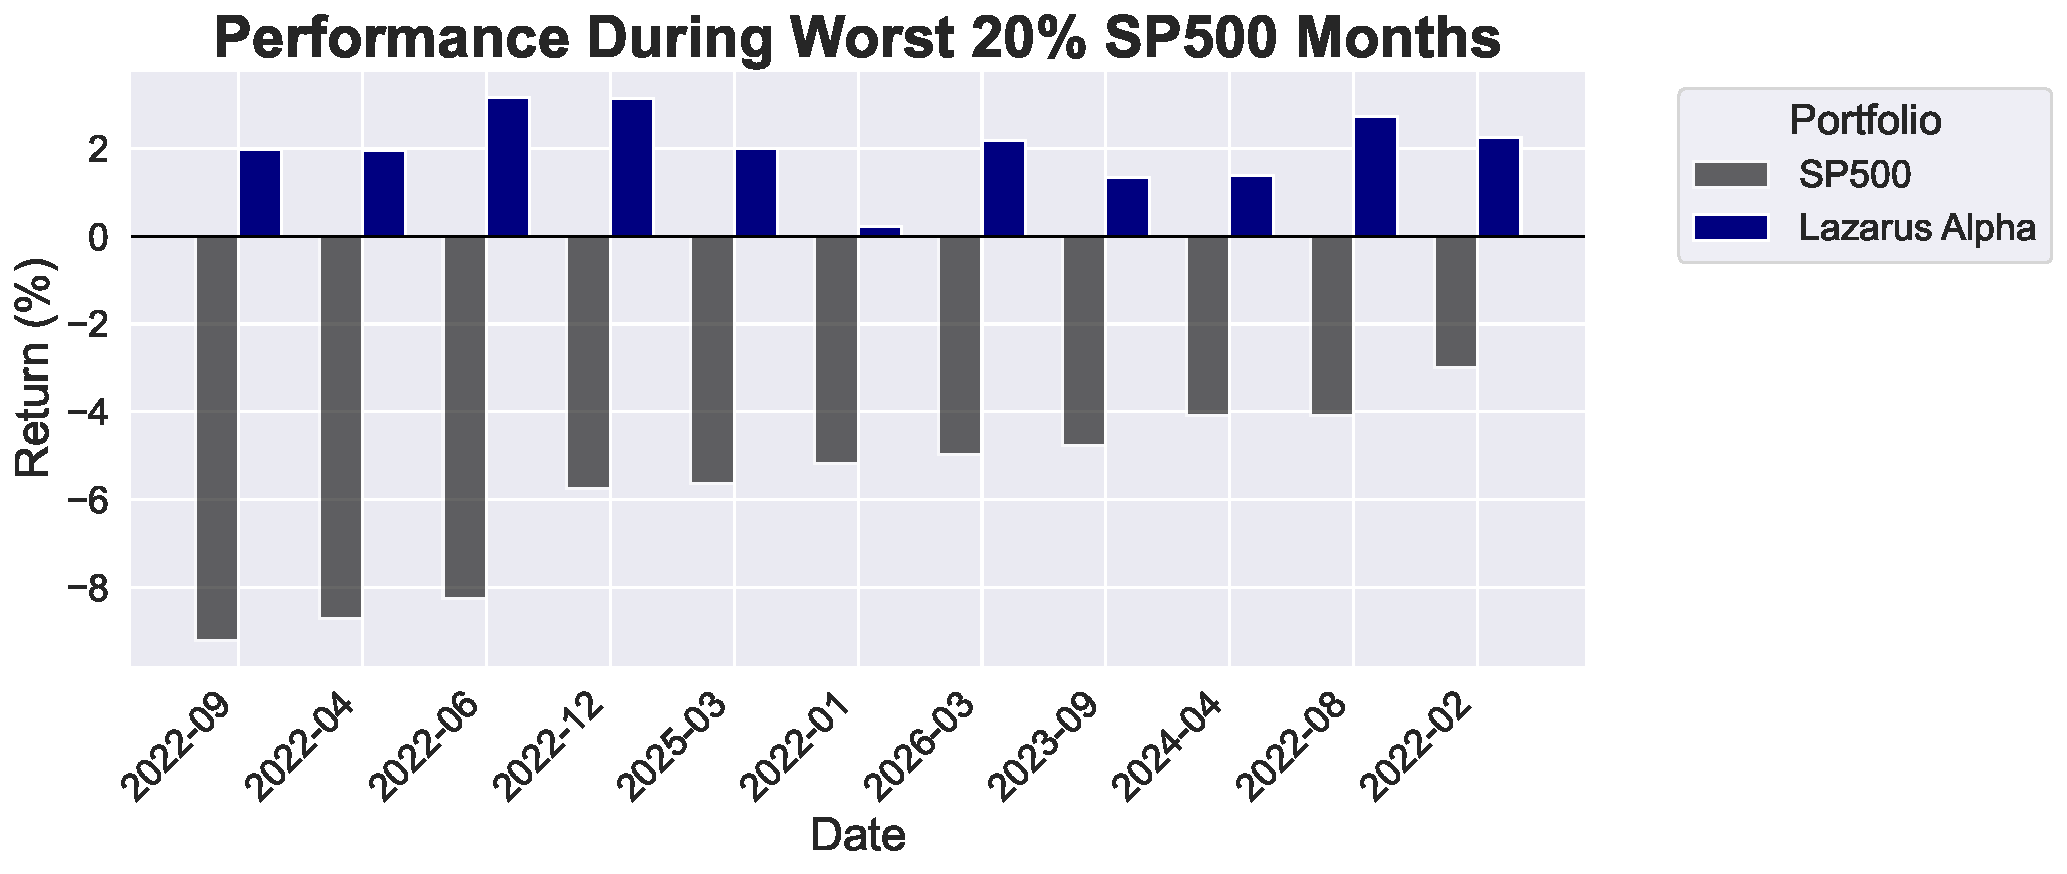
\includegraphics[width=0.8\textwidth]{../../lazarus/worst20_sp500_6m_reb.pdf}
    \caption{Portfolio performance during the 20 worst months for the S\&P 500.}
    \label{fig:worst_sp500}
\end{figure}

By thoughtfully aggregating aggressive, strictly non-correlated return streams and enforcing severe risk limits, we deliver a product that mathematically and empirically transcends the risk-return profile of any single asset.

\end{document}
